\documentclass[../physics12.tex]{subfiles}
\graphicspath{{\subfix{../figures/}}}
\begin{document}
\chapter{Geometric Optics}
\section{Formulas}
Check chapter 13 formulas.

\section{Two Mirrors Problem}
The reflecting surfaces of two intersecting flat mirrors are at an angle of $56\degree$. A light ray strikes the horizontal mirror at an angle of $53\degree$ with respect to the mirror's surface.
\begin{center}
    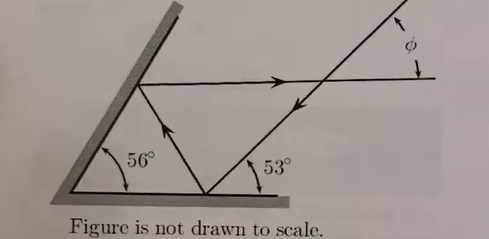
\includegraphics[width=0.5\textwidth]{14.1.PNG}
\end{center}
Calculate the angle of $\varphi$. Answer in units of $\degree$.

\section{Liquid in a Cistern Problem}
A cylindrical cistern, constructed below ground level, is 3 m in diameter and 2.2 m deep and is filled to the brim with a liquid whose index of refraction is 1.52. A small object rests on the bottom of the cistern at its center.
\begin{center}
    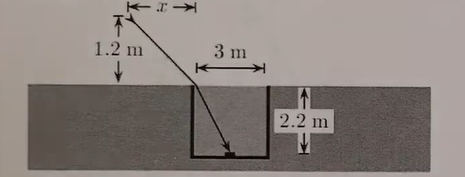
\includegraphics[width=0.5\textwidth]{14.2.PNG}
\end{center}
How far $x$ from the edge of the cistern can a girl whose eyes 1.2 m from the ground stand and still see from the object? Answer in units of m.

\section{Silica Prism Problem}
Light of wavelength 700 nm is incident on the face of a silica prism at an angle of $\theta_1 = 75\degree$ (with respect to the normal to the surface).
The apex angle of the prism is $\varphi = 60\degree$. The value of the index of refraction for silica is $n=1.455$.
\begin{center}
    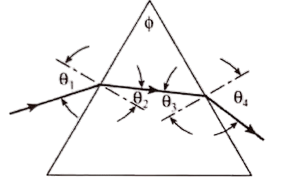
\includegraphics[width=0.5\textwidth]{14.3.PNG}
\end{center}
(a) Find the angle of refraction at this first surface. Answer in units of degrees.

(b) Find the angle of incidence at the second surface. Answer in units of degrees.

(c) Find the angle of refraction at the second surface. Answer in units of degrees.

(d) Find the angle between the incident and emerging rays. Answer in units of degrees.

\section{Two Beams in Glass Problem}
A certain kind of glass has an index of refraction of 1.65 for blue light of wavelength 430 nm and an index of 1.615 for red light of wavelength 680 nm. A beam containing these two colors 
is incident at an angle of $30\degree$ on a piece of this glass.

What is the angle between the two beams inside the glass? Answer in units of $\degree$.
\end{document}